\documentclass[fleqn]{article}
\usepackage[UTF8]{ctex}
\usepackage{listings}
\usepackage{diagbox}
\usepackage[german]{babel}
\usepackage[T1]{fontenc}
\usepackage[latin1]{inputenc}
\usepackage{titlesec}
\usepackage{geometry}
\usepackage{qtree}
\usepackage{tikz}
\usepackage{extarrows}
\usepackage{amsmath}
\usepackage{amssymb}
\setcounter{secnumdepth}{0}
\usetikzlibrary{positioning}
\geometry{top=2.5cm, bottom=2.5cm}
\lstset{
 columns=fixed,       
 numbers=left,                                        % 在左侧显示行号
 numberstyle=\tiny\color{gray},                       % 设定行号格式
 frame=none,                                          % 不显示背景边框
 backgroundcolor=\color[RGB]{245,245,244},            % 设定背景颜色
 keywordstyle=\color[RGB]{40,40,255},                 % 设定关键字颜色
 numberstyle=\footnotesize\color{darkgray},           
 commentstyle=\it\color[RGB]{0,96,96},                % 设置代码注释的格式
 stringstyle=\rmfamily\slshape\color[RGB]{128,0,0},   % 设置字符串格式
 showstringspaces=false,                              % 不显示字符串中的空格
 language=c++,                                        % 设置语言
 breaklines,                                          % 自动换行
}

%\title{TU Chemnitz \\ Praktikum}

%\author{Gr\\ Dongze Yang}

\begin{document}

%\maketitle

\newpagestyle{main}{
    \sethead{}{}{Math IV}
    \setfoot{}{\thepage}{}
    \headrule
    \footrule
}
\pagestyle{main}

\section{Vektoranalysis}

$$Vektorfeld\quad v:\begin{pmatrix}
    v_1(x_1,x_2,x_3)\\v_2(x_1,x_2,x_3)\\v_3(x_1,x_2,x_3)
\end{pmatrix}$$

\noindent 1. $rot(v)=\begin{pmatrix}
    \partial_1\\\partial_2\\\partial_3
\end{pmatrix}\times\begin{pmatrix}
    v_1(x)\\v_2(x)\\v_3(x)
\end{pmatrix}=\begin{pmatrix}
    \frac{\partial v_3}{\partial x_2}-\frac{\partial v_2}{\partial x_3}\\
    \frac{\partial v_1}{\partial x_3}-\frac{\partial v_3}{\partial x_1}\\
    \frac{\partial v_2}{\partial x_1}-\frac{\partial v_1}{\partial x_2}
\end{pmatrix}=\nabla\times\vec{v}$

\noindent 2. 向量$\vec{v}$的维度$n$(即$\mathbb{R}^n$上的$n$)=$div(\vec{v})$

$div(\vec{v})=\nabla(\vec{v})\cdot \vec{v}=\sum_{i=1}^n\frac{\partial v_i}{\partial x_i}$,即一阶导数之和。

\begin{center}
    \begin{tabular}{l||l}
        \hline
        Rotation旋度&Divergenz散度\\
        \hline
        $rot(\nabla v)=\vec{0}$&$div(rot(\vec{v}))=0$\\
        \hline
        $rot(\phi\cdot\vec{v})=\nabla\phi\times\vec{v}+\phi\cdot rot(\vec{v})$&$div(\nabla\phi)=\Delta\phi$\\
        \hline
        $rot(rot(\vec{v}))=\nabla(div(\vec{v}))-\Delta\vec{v}$&$div(\phi\cdot\vec{v})=\vec{v}\cdot\nabla\phi+\phi(div(\vec{v}))$\\
        \hline
    \end{tabular}
\end{center}

$\vec{w}$ 被称为$\vec{v}$的矢量势(Vektorpotential): $\vec{v}=rot(\vec{w})$。

求$div(\vec{v})$,若$\vec{v}$的形式比较复杂,那么可以考虑使用上面的替换形式,使$div(\vec{v})$项能够被化简出来,由此得出结果。
例如求$\frac{\vec{x}}{\|\vec{x}\|}$的$div=div(\|\vec{x}\|^{-1}\cdot\vec{x})$,然后用上面第三个替换计算即可。
\\
\\
\noindent 3. $\Delta$, Laplace-Operator : $\Delta f=\frac{\partial^2 f}{\partial x_1^2}+\frac{\partial^2 f}{\partial x_2^2}+...+\frac{\partial^2 f}{\partial x_n^2}=\sum_{i=1}^{n}\frac{\partial^2 f}{\partial x_i^2} $,即二阶导数之和。

计算方法也是用上面的替换式。需要分离出$div(\vec{x})$项,此项$=n$。
\\
\\
\noindent 4. Symmetrische Jacobi-Matrix 对称雅可比矩阵

对于向量场$v(x,y)$,求其$J$矩阵$=\begin{pmatrix}
    J_{11} & J_{12}\\
    J_{21} & j_{22}
\end{pmatrix}=\begin{pmatrix}
    \frac{\partial v_1}{\partial x} & \frac{\partial v_1}{\partial y}\\
    \frac{\partial v_2}{\partial x} & \frac{\partial v_2}{\partial y}
\end{pmatrix}$

若$J_{11}=-J_{22}$及$J_{12}=J_{21}$,则对称。

类似的,可以把虚数中的实部$Re$看做向量场中的$v_1$,把虚部$Im$看做$v_2$,并借此关系来判断是否可微(differenzierbar)。

\noindent 5. 判断某Vektorfeld $\vec{v}$是否有Vektorpotential $\vec{w}$。已知$v(x)=\begin{bmatrix}
    y\\z\\x
\end{bmatrix}$,$\vec{v}=rot(\vec{w})$。

设$\vec{w}=\begin{bmatrix}
    w_1\\w_2\\w_3
\end{bmatrix}$,则有$rot(\vec{w})=\begin{pmatrix}
    \frac{\partial w_3}{\partial y} - \frac{\partial w_2}{\partial z}\\
    \frac{\partial w_1}{\partial z} - \frac{\partial w_3}{\partial x}\\
    \frac{\partial w_2}{\partial x} - \frac{\partial w_1}{\partial y}
\end{pmatrix}$,令$w_3=c\, (const)$,则有:

$v_1=y=\frac{\partial w_3}{\partial y} - \frac{\partial w_2}{\partial z}=0-\frac{\partial w_2}{\partial z}\Rightarrow w_2=\int -y dz=-yz+A$

$v_2=z=\frac{\partial w_1}{\partial z} - \frac{\partial w_3}{\partial x}=\frac{\partial w_1}{\partial z}-0\Rightarrow w_1=\int z dz=\frac{1}{2}z^2+B$

$v_3=x=\frac{\partial w_2}{\partial x} - \frac{\partial w_1}{\partial y}\Leftrightarrow \frac{\partial (-yz+A)}{\partial x}-\frac{\partial (\frac{1}{2}z^2+B)}{\partial y}=A'+0\Rightarrow A=\int xdx=\frac{1}{2}x^2,B=0$

$\therefore w_2=-yz+\frac{1}{2}x^2,w_1=\frac{1}{2}z^2,w_3=0$

\clearpage
\section{Intergralsätze}

\noindent 1. Satz von Green 格林公式:$\int_B[\frac{\partial v_2}{\partial x}-\frac{\partial v_1}{\partial y}]dV$

1.1 Flächeninhaltsformel($F(B)$ des Bereiches B die Formel): $F(B)=\frac{1}{2}\int_{t_a}^{t_b}[-y(t)\cdot x'(t)+x(t)\cdot y'(t)]$

% 1.2 边际曲线(positiv orientierter Randkurve)$r(t)=\begin{pmatrix}
%     x(t)\\y(t)
% \end{pmatrix}$的单位法向量(Einheitsnormalenvektor,在$\partial B$上) $\vec{n}(t)=\frac{1}{\|r'(t)\|}\cdot\begin{pmatrix}
%     y'(t)\\-x'(t)
% \end{pmatrix}$。曲线的矢量场/向量场$\vec{v}=\begin{pmatrix}
%     v_1\\v_2
% \end{pmatrix}=\begin{pmatrix}
%     -\frac{\partial x(t)}{\partial y}\\\frac{\partial x(t)}{\partial x}
% \end{pmatrix}$,向量场的

1.2 应用:第二类曲线积分-求做功。对于一个曲线$\gamma$,求向量场$\vec{v}$在这之上的做功:

-$W=\int_{x_0}^{x_1} \int_{y_0}^{y(x)}[\frac{\partial v_2}{\partial x}-\frac{\partial v_1}{\partial y}]dydx$,也等于1.1

\noindent 2. 可能用到的三角转换

\begin{center}
    \begin{tabular}{l|l||l|l||l|l}
        \hline
        $sec(x)$&$c/b$&$sin(\pi+x)$&$-sin(x)$&$tan(x+y)$&$\frac{tan(x)+tan(y)}{1-tan(x)tan(y)}$\\
        \hline
        $cot(x)$&$b/a$&$cos(\pi+x)$&$-cos(x)$&$cot(x+y)$&$\frac{cot(x)cot(y)-1}{cot(y)+cot(x)}$\\
        \hline
        $csc(x)$&$c/a$&$tan(\pi+x)$&$tan(x)$&$sin(x)+sin(y)$&$2sin(\frac{x+y}{2})cos(\frac{x-y}{2})$\\
        \hline
        $sin^2(x)$&$1-cos(x)$&$cos(\pi+x)$&$cos(x)$&$cos(x)+cos(y)$&$2cos(\frac{x+y}{2})cos(\frac{x-y}{2})$\\
        \hline
        $1+tan^2(x)$&$sec^2(x)$&$tan(x)+tan(y)$&$\frac{sin(x+y)}{cos(x)cos(y)}$\\
        \hline
        $1+cot^2(x)$&$csc^2(x)$&$sin(x)cos(x)$&$\frac{1}{2}sin(2x)$\\
        \hline
        
    \end{tabular}
\end{center}

\noindent 3. 分部积分$\int u'v ds = uv-\int uv' ds$

\noindent 4. Oberflächenintegral/Flussintegral 表面积分/流积分: $\int_{\vec{\phi}}f(\vec{v})dO$,$\int_{S}\vec{v}d\vec{O}$

表面为$\vec{\phi}=\begin{pmatrix}
    x(u,v)\\y(u,v)\\z(u,v)
\end{pmatrix}$,$dO=\|\vec{t_{u}}(u,v)\times\vec{t_{v}}(u,v)\|dudv$,其中$\vec{t_u}=\nabla\phi_u$,$\vec{t_v}=\nabla\phi_v$

表面的单位法向量Einheitsnormalenvektor: $\vec{n}=\frac{\vec{t_{u}}(u,v)\times\vec{t_{v}}(u,v)}{\|\vec{t_{u}}(u,v)\times\vec{t_{v}}(u,v)\|}$

Oberflächenintegral/Flussintegral des stetigen Vektorfeldes 连续向量场的表面积分/流积分: $$\int_{S}\vec{v}d\vec{O}=\int_{\vec{\phi}}\vec{v}(\vec{x})\cdot\vec{n}(\vec{x})dO$$

-即向量场$\vec{v}$沿着方向$\vec{n}$通过表面$S$的流量Fluss。

\noindent 5. 已知面$S(\varphi,\theta)=\begin{pmatrix}
    \sqrt{2}cos(\varphi)sin(\theta)\\\sqrt{2}sin(\varphi)sin(\theta)\\\sqrt{2}cos(\theta)
\end{pmatrix},\,\varphi\in[0,2\pi],\theta\in[0,\frac{\pi}{4}]$,场$\vec{v}$有向量势$\vec{w}=\begin{pmatrix}
    xz,xy,yz
\end{pmatrix}$,求流量。

\begin{center}
    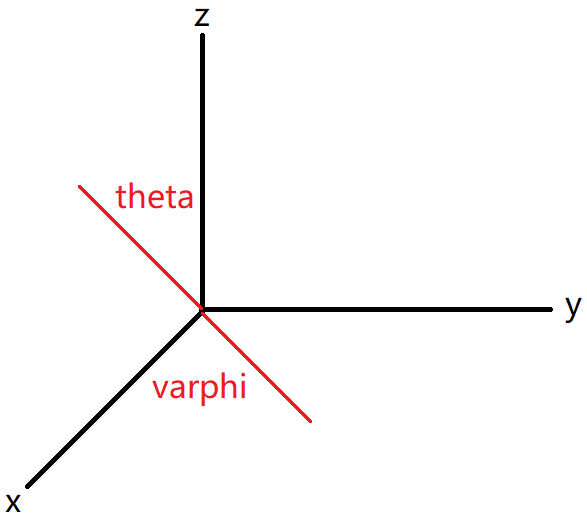
\includegraphics[scale=0.2]{bild1.png}
\end{center}

解:目的是计算$f=\iint_F\vec{v}\cdot \pmb{n_0}dF=\iint_B\vec{v}(P(u,v))\cdot \pmb{n}(u,v)d(u,v)$

a. 若面S未参数化,需要先将S参数表示parametrisieren。

b. $\pmb{n}(u,v)=\pmb{n}(\varphi,\theta)=\frac{\partial S}{\partial x}\times\frac{\partial S}{\partial y}=\begin{pmatrix}
    -\sqrt{2}sin(\varphi)sin(\theta)\\\sqrt{2}cos(\varphi)sin(\theta)\\0
\end{pmatrix}\times\begin{pmatrix}
    \sqrt{2}cos(\varphi)cos(\theta)\\\sqrt{2}sin(\varphi)cos(\theta)\\-\sqrt{2}sin(\theta)
\end{pmatrix}=\begin{pmatrix}
    2cos(\varphi)sin^2(\theta)\\-2sin(\varphi)sin^2(\theta)\\-2sin(\theta)cos(\theta)
\end{pmatrix}$

c. 把参数化表示的$x,y,z$带入$\vec{v}$中: $\vec{v}(P(u,v))=\vec{v}(S(\varphi,\theta))$

\qquad 对于此题有$\vec{v}(S(\varphi,\theta))=rot(\vec{w})=\begin{pmatrix}
    z\\x\\y
\end{pmatrix}=\begin{pmatrix}
    \sqrt{2}cos(\theta)\\\sqrt{2}cos(\varphi)sin(\theta)\\\sqrt{2}sin(\varphi)sin(\theta)
\end{pmatrix}$

d. 化简$\vec{v(S(\varphi,\theta))}\cdot \pmb{n}(\varphi,\theta)$

$\begin{pmatrix}
    \sqrt{2}cos(\theta)\\\sqrt{2}cos(\varphi)sin(\theta)\\\sqrt{2}sin(\varphi)sin(\theta)
\end{pmatrix}\cdot \begin{pmatrix}
    2cos(\varphi)sin^2(\theta)\\-2sin(\varphi)sin^2(\theta)\\-2sin(\theta)cos(\theta)
\end{pmatrix}$

$=2\sqrt{2}[sin(\varphi)sin^2(\theta)cos(\theta)-sin(\varphi)cos(\varphi)sin^3(\theta)-sin(\varphi)sin^2(\theta)cos(\theta)]$

$=-\sqrt{2}sin(2\varphi)sin^3(\theta)$

e. 带入公式,解得

$$\int_0^{\frac{\pi}{4}}\int_0^{2\pi}-\sqrt{2}sin(2\varphi)sin^3(\theta)d\theta d\varphi = 0$$

\clearpage
\section{Komplexe Funktionen und Differenzierbarkeit}

$$f(z)=f(x+iy)=Re+Im\cdot i$$

\noindent 0. 可能用上的转换

\begin{center}
    \begin{tabular}{l|l||l|l||l|l}
        $r=|z|$&半径为r圆&$\overline{z-w}$&$\bar{z}-\bar{w}$&$\overline{zw}$&$\bar{z}\bar{w}$\\
        \hline
        $\bar{z}$&$x-yi$&$\overline{(\frac{z}{w})}$&$\frac{\bar{z}}{\bar{w}}$&$|z|^2$&$z\bar{z}$\\
        \hline
        $z^{-1}$&$\bar{z}|z|^{-2}$&$f(\bar{z})$&$\overline{f(z)}$&$sinh(x)$&$-i\cdot sin(ix)$
    \end{tabular}

    \begin{tabular}{c|c}
        \hline
        Form & 形如 \\
        \hline
        algebraischen Form & $z=x+yi$  \\
        \hline
        Polarform &$z=r(cos\varphi +i\cdot sin\varphi)$\\
        \hline
        Exponentialform & $re^{i\varphi}$\\
        \hline
    \end{tabular}
    $\varphi = \left\{
        \begin{aligned}
            arctan(\frac{y}{x}) &, x>0\\
            arctan(\frac{y}{x})+\pi &, x<0,y\geq 0\\
            arctan(\frac{y}{x})-\pi &, x<0,y<0\\
            \frac{\pi}{2} &, x=0, y>0\\
            -\frac{\pi}{2} &, x=0, y<0\\
            undefined &, x=0, y=0
        \end{aligned}
        \right.$
\end{center}

\qquad $x=rcos\varphi,\, y=rsin\varphi\rightarrow r=\sqrt{x^2+y^2}=\sqrt{\Re^2+\Im^2}$
. $tan\varphi = \frac{\Im}{\Re}$

\qquad $z^n=r^n(cos(n\varphi) + i\cdot sin(n\varphi)) = r^ne^{ni\varphi}$

\qquad 一般4次根号下就相当于把角度转3次,一次转$\frac{\pi}{2}$。

\textbf{泰勒级数(Summenfunktion):}
\begin{center}
    $
        \begin{aligned}
            \frac{1}{1-x} &=1 + x + x^2 +x^3 +...=\sum_{n=0}^{\infty}x^n, \, x\in (-1,1)\\
            e^x &= 1+x+\frac{x^2}{2!}+\frac{x^3}{3!}+...+\frac{x^n}{n!} = \sum_{n=0}^{\infty}\frac{x^n}{n!}, \, x\in\mathbb{R}\\
            cos(x) &= 1-\frac{x^2}{2!}+\frac{x^4}{4!}-\frac{x^6}{6!}+\frac{x^8}{8!}-...=\sum_{n=0}^{\infty}(-1)^n\frac{x^{2n}}{(2n)!},\, x\in\mathbb{R}\\
            sin(x) &= x-\frac{x^3}{3!}+\frac{x^5}{5!}-\frac{x^7}{7!}+\frac{x^9}{9!}-...=\sum_{n=1}^{\infty}(-1)^{n-1}\frac{x^{2n-1}}{(2n-1)!}=\sum_{n=0}^{\infty}(-1)^{n}\frac{x^{2n+1}}{(2n+1)!},\, x\in\mathbb{R}\\
            ln(1+x)&= x-\frac{x^2}{2}+\frac{x^3}{3}-\frac{x^4}{4}+\frac{x^5}{5}-...=\sum_{n=1}^{\infty}(-1)^{n-1}\frac{x^n}{n}=\sum_{n=0}^{\infty}(-1)^{n+1}\frac{x^n}{n},\, x\in (-1,1]\\
            tan^{-1}(x)&= x-\frac{x^3}{3}+\frac{x^5}{5}-\frac{x^7}{7}+\frac{x^9}{9}-...=\sum_{n=1}^{\infty}(-1)^{n-1}\frac{x^{2n-1}}{2n-1}=\sum_{n=0}^{\infty}(-1)^{n}\frac{x^{2n+1}}{2n+1},\, x\in[-1,1]
        \end{aligned}
    $
\end{center}

\textbf{用欧拉公式(Eulerschen Formel)表示正余弦:}

$$cos(kx)=\frac{e^{ikx}+e^{-ikx}}{2},\, sin(kx)=\frac{e^{ikx}-e^{-ikx}}{2i},e^{ikx}=cos(kx)+isin(kx)$$



\noindent 1. 求$f'(z)$(及判断是否为holomorph)

a. 先判断$f(z)$是否可导:若$Re_x == Im_y$且$Re_y == -Im_x$,此时为holomorph(纯的),则可导。

b. 当可导,要想办法用$z$替换$x+iy$,最终使式子中的变量只有$z$。可用到复数变换。

已知:
\begin{center}
    \begin{tabular}{l|l||l|l}
        $f(z)$&$f'(z)$&$f(z)$&$f'(z)$\\
        \hline
        $z^2$&$2z$&$e^y(sin(x)+i\cdot cos(x))$&$e^{y-ix}=e^{-iz}$\\
        \hline
        $|z|^2$&$\times$&$\frac{1}{z}$&$-\frac{1}{z^2}$\\
        \hline
        $zRe(z)$&$\times$&$sin(z)$ and $cos(z)$&$cos(z)$ and $-sin(z)$\\
        \hline
        $sinh(x)$&$cosh(x)$&$cosh(x)$&$sinh(x)$
    \end{tabular}
\end{center}

\noindent 2. 判断$u(x,y)$是否为harmonische Funktion,若是,求其komplexe Potential

a. 用拉普拉斯运算: 若$\Delta u = div(\nabla u)=0$,则是。

b. 若是,则需要求其级数$f = u + v\cdot i$是holomorph的。则$u_x=v_y$且$u_y=-v_x$。那么可以用积分求得$v$的值。带入$f$即可。

\section{Komplexes Integral}

$$\int_Kf(z)dz=\int_{\gamma}f(z)\cdot z'dz=\int_{\gamma}x\cdot x'dt + i\cdot\int_{\gamma}x\cdot y'dt$$

\noindent 注意!形如$\int_KRe\,zdz$的$Re\,z$为上式中的$f(z)$

\noindent 1. 具体计算(计算过程类似求流量Seite 2-5)

a. 先将路径K用参数方程表示出来,为$f(z)=Re(t)+Im(t)\cdot i$。

\qquad bsp1. 单位圆:$f(z)=cos(t)+sin(t)\cdot i$

\qquad bsp2. 从0到1到$1-i$:$f_1(z)=0+t\cdot i$,$f_2(z)=1-i,t\in[0,1]$

b. 判断$f(z)$是否为holomorph的: $Re_x == Im_y \,?\, Ja, Nein $

c-1. 若不是holomorph的,则直接用公式计算。在计算时,$i$为一个常量。

c-2. 若是,

\noindent 2. Cauchysche Integralsatz

求$f(z)=\frac{1}{z}$的积分

(1) 若路径为$K: |z-1-i|=1$。

可知$K$描述的是一个圆心为(1+i),半径为1的圆,因为$|z-z_0|=r$,其中$z_0=a+bi$,则圆心为(a,b)。
这是一个平滑的闭合曲线,因此根据Cauchysche Integralsatz可知积分=0。

(2) 若路径为$K=\{z=x+iy,x=cos^3\varphi,y=sin^3\varphi,\varphi\in[0,2\pi]\}$

图形为一个闭合的星形线,即不是平滑的闭合曲线,因此不能用Cauchysche Integralsatz,而是需要用Cauchysche Integrationsformel计算。

\noindent 3. Cauchysche Integrationsformel

$$f(a)=\frac{1}{2\pi i}\int\frac{f(z)}{z-a}dz=Res(f,0)$$

$$f^{(n)}(a)=\frac{1}{2\pi i}\int\frac{f^{(n)}(z)}{z-a}dz$$

$$f^{(n)}(a)=\frac{n!}{2\pi i}\int\frac{f(z)}{(z-a)^{n+1}}dz$$

bsp: $\int_K\frac{-icos(z)}{z}dz$ mit $K:|z-2|=3$

正常求法(利用泰勒级数替换):

\qquad $\frac{-icos(z)}{z}=\frac{-i\sum_{k=0}^{\infty}(-1)^k\frac{z^{2k}}{(2k)!}}{z}=-i\sum_{k=0}^{\infty}(-1)^k\frac{z^{2k-1}}{(2k)!}=-i\sum_{k=-1}^{\infty}(-1)^{k+1}\frac{z^{2k+1}}{(2k+2)!}$

\qquad $\Rightarrow a_{-1}=-i(-1)^0=-i=Res(f,0),\therefore \int = 2\pi i \cdot (-i)=2\pi$

利用Residuensatz:

$$Res_{z_0}f=\frac{g^{(m-1)}(z_0)}{(m-1)!}$$

$$f(z)=(z-z_0)^{-m}g(z)$$

\qquad 把被积函数化成上述形式:$\frac{-icos(z)}{z}= (z-0)^{-1}\cdot(-icos(z))$。

\qquad 所以$m=1,m-1=0,z_0=0,g(z)=-icos(z)$。带入,则有$Res\,f=\frac{g^0(0)}{0!}=-i$。

\section{Laurentreihen und Residuensatz}

\noindent 1. Laurentreihen

$$f(z)=\sum_{k=-\infty}^{\infty}a_kz^k, a_k\in(c,d)$$

bsp. $f(z)=\frac{1}{z(z-1)},|z-1|\in(0,1)$

则:$f(z)=\frac{1}{z}\cdot\frac{1}{z-1}=\frac{1}{z-1}\cdot\frac{1}{1-(1-z)}\rightarrow$

(配合泰勒级数)$=\frac{1}{z-1}\sum_{k=0}^{\infty}(1-z)^{k}=\frac{1}{z-1}\sum_{k=0}^{\infty}(-1)^{k}(z-1)^{k}$

\qquad $=\sum_{k=0}^{\infty}(-1)^{k}(z-1)^{k-1}=\sum_{k=-1}^{\infty}(-1)^{k+1}(z-1)^{k}$

\qquad 这就是Laurentreihen。


\section{Kombinatorik und Ereignisalgebra}

\noindent $A_n^k$: 排列 = $\frac{n!}{(n-m)!}$。全排列$=n!$

重复排列:$=n^m$。当样本可以重复抽取时。

\noindent 1. 如从1到100 000的所有正整数中,至少有一位包含1的正整数有多少个?

正整数个数共有$10000=10^5$个,所有不包含1的数字有$9^5$个,但这中包含了一种情况
是00000,不在区间内,因此要去掉。那么包含1的正整数为:$10^5-9^5+1$。
\\
\\
\noindent 2. 有7封信,随意投入3个信箱,有多少种投法?

第一封信有3中,第二封有三种……所以共有$3^7$种。

\noindent 3. 有5对夫妻参加婚礼,被安排在一张10座圆桌,求5对夫妻恰好相邻而坐的概率。

我们只需要让任意一人坐下,他/她的夫/妻的位置也确定了。接下来只需要给剩下的4对夫妻全排列即可。则排列为$A_4^4$

\noindent 4. a,b,c,d,e围着一张圆桌。

a) 共有多少种?有$(5-1)!=24$种

b) a,b相邻多少种?a在b左边$(5-2)!=6$,a在b右边$(5-2)!=6$,则共有12种。

c) a,b不相邻有多少种?24-12=12种。

\noindent $C_n^k=\begin{pmatrix}
    n\\k
\end{pmatrix}$: 组合$=\frac{n!}{k!(n-k)!}$。从$n$个样本中不重复抽出$k$个,不管其顺序组成一组

重复组合:从n个样本中重复抽取k个样本。$H_n^k=\frac{(n+k-1)!}{k!(n-1)!}$

\noindent 5. 15条路,每条路上两种颜色,可以是相同颜色,问至少需要多少种颜色可以使所有路区分开?

假设需要n种颜色,此题为重复组合——即颜色的组合。那么有$H_n^2=15$,解得$n=5$。

\section{Wahrscheinlichkeit \& Verteilungen}

$P(A\cup B)=P(A)+P(B)-P(A\cap B)$

$P(A|B)=\frac{P(A\cap B)}{P(B)}$

\noindent 1. unabhängig bzw. disjunkt? 独立或不相交

$P(A\cap B) = P(A)\cdot P(B)$, $P(A|B)=P(A)$

\noindent 2. 分布总结


\begin{center}
    2.1离散分布
    \begin{tabular}{l|l|l|l|l}
        \hline
        名称&表示&概率/密度&期望&方差\\
        \hline
        Bernoulli/两点/0-1&$\Omega=\{0,1\}$&成功为$p$,失败为$1-p$&$p$&$p(1-p)$\\
        \hline
        Binomial/二项分布&$X\sim B(n,p)$&$P(X=k)=C_n^kp^kq^{n-k}$&$np$&$np(1-p)$\\
        \hline
        Hypergeometrische&$X\sim H(n,K,N)$&$P(X=k)=\frac{C_K^kC_{N-K}^{n-k}}{C_N^n}$&$n\frac{K}{N}$&$n\frac{K}{N}\frac{(N-K)}{N}\frac{N-n}{N-1}$\\
        \hline
        Poisson/泊松&$X\sim P(\lambda)$&$P(X=k)=\frac{e^{-\lambda}\lambda^k}{k!}$&$\lambda$&$\lambda$\\
        \hline
    \end{tabular}
\end{center}

二项分布:重复进行n次独立试验,每次成功的概率为$p$,总计成功的次数为$k$。当n=1时,为0-1分布。

超几何:有$N$个样本,不归还抽出$n$个,成功抽出指定样本的个数。如有$N$个样本,其中$K$个是不合格的,抽出$n$个,其中$k$个是不合格的概率。若$n=1$,则等同Bernoulli分布。

泊松:$\lambda$是单位时间/面积内,随机事件的平均发生率。描述时间单位内,随机事件发生的次数的概率。如某设施在一定时间内收到的服务请求的次数;车站候车人数;机器出现故障数;自然灾害次数。

\begin{center}
    2.2连续分布
    \begin{tabular}{l|l|l|l|l|l}
        \hline
        名称&表示&概率/密度$f(x;\lambda)$&累积$F(x;\lambda)$&期望&方差\\
        \hline
        Exponential/指数&$X\sim E(\lambda)$&$
        \left\{
            \begin{array}{lr}
                \lambda e^{-\lambda x} &, x\geq 0\\
                0 &, x<0
            \end{array}
        \right.
        $&$
        \left\{
            \begin{array}{lr}
                1- e^{-\lambda x} &, x\geq 0\\
                0 &, x<0
            \end{array}
        \right.$&$\lambda^{-1}$&$\lambda^{-2}$\\
        \hline
        Normal-/Gauß-V&$X\sim N(\mu,\sigma^2)$&$f(x)=\frac{1}{\sigma\sqrt{2\pi}}e^{-\frac{(x-\mu)^2}{2\sigma^2}}$&$P(X\leq x)=\Phi(\frac{x-\mu}{\sigma})$&$\mu$&$\sigma^2$\\
        \hline
        Gleich-均匀&$X\sim U[a,b]$&$f(x)
        \left\{
            \begin{array}{lr}
                \frac{1}{b-a} &, x\in[a,b]\\
                0 & sonst
            \end{array}
        \right.$&$F(x)
        \left\{
            \begin{array}{lr}
                \frac{x-a}{b-a} &, x\in[a,b)\\
                0 & sonst
            \end{array}
        \right.$&$\frac{a+b}{2}$&$\frac{(b-a)^2}{12}$\\
        \hline
    \end{tabular}
\end{center}

指数分布:$P(X\leq x)=F(x),P(X\geq x)=1-F(x)$

正态分布:同上。
\\
\\
\noindent 3. 期望与方差

离散:$E(x)=\sum_{i=1}^nx_i\cdot p_i$

连续:$E(x)=\int_{-\infty}^{\infty}x\cdot f(x)dx$

$E(aX+bY)=aE(X)+bE(Y)$

$V(x)=E(x^2)-E^2(x)$

$V(x)=E[(x-\mu)^2]$,其中$\mu$为期望值。

$V(x)=Cov(x,x)$

离散:$V(x)=\sum_{i=1}^np_i\cdot(x_i-\mu)^2=\sum_{i=1}^n(p_i\cdot x^2)-\mu^2$。
当$x$的概率相等时:$V(x)=\frac{\sum x_i^2}{n}-\mu^2$。

连续:$V(x)=\int(x-\mu)^2f(x)dx = \int x^2f(x)dx-\mu^2$

$V(x+a)=V(x)$

$V(aX)=a^2V(X)$

$V(aX=bY)=a^2V(X)+b^2V(Y)+2ab\cdot Cov(X,Y)$

$V(X-Y)=V(X)+V(Y)-2Cov(X,Y)$

$V(\sum X_i)=\sum_{i,j=1}^NCov(X_i,X_j)=\sum_{i=1}^NV(X_i)+\sum_{i\neq j}Cov(X_i,Y_i)$

\noindent 4. 当某些数据符合某种分布$f$时,若要求“至少需要多少X,使得a\%的事件能够完成”.

此时求的就是$P(X\leq n)\geq a\%$或$P(X\geq n)= a\%$中的$n$,带入相关的累积函数即可求得。

\noindent 5. 概率密度函数一定符合条件$\int_{-\infty}^{\infty} f(x)dx=1,\,f(x)\geq 0$。

\noindent 6. 对于高斯分布,有$x\geq 0\rightarrow F(x)=\Phi(x)=1-\Phi(-x)$,$P(X>0)=1-P(X\leq 0)$























































































































\end{document}